\documentclass[a4paper,12pt]{article}

\usepackage[utf8]{inputenc}
\usepackage[T1]{fontenc}
\usepackage{amsmath}
\usepackage{graphicx}
\usepackage{hyperref}
\usepackage{geometry}
\usepackage{subcaption}
\usepackage{float}
\usepackage{booktabs}
\usepackage{array}
\usepackage{xcolor}
\usepackage{enumitem}
\usepackage[american]{circuitikz}

\geometry{margin=1in}

\hypersetup{
    colorlinks=true,
    linkcolor=blue,
    citecolor=blue,
    urlcolor=blue,
}

\title{\textbf{IR Transmission Research for Multi-Transmitter Systems}}
\author{}
\date{}

\begin{document}

\maketitle

% ============================================================
% ABSTRACT
% ============================================================

\begin{abstract}

This research investigates infrared (IR) transmission in a
multi-transmitter system using the NEC communication protocol.
The system operates with a 38 kHz carrier and 940 nm infrared radiation.
Interference was observed when multiple transmitters were placed close
to one another, motivating investigation of transmitter directivity,
optical coverage, and isolation.

The receiver system consists of a \(12 \times 12\) array of individual
IR receivers occupying a total area of approximately
\(900\,\text{cm}^2\), corresponding to a
\(30\,\text{cm} \times 30\,\text{cm}\) receiving surface.
The expected transmitter-to-receiver separation is approximately
1--2 m.

Testing with a KY-005 transmitter showed insufficient optical coverage
for reliable reception across the complete receiver array.
A directional 940 nm transmitter using Vishay TSAL6200 infrared
emitters is therefore proposed. The transmitter uses two series-connected
IR LEDs as its basic optical source and can be expanded to four LEDs
using a second independently current-limited branch.

An AO3400A logic-level N-channel MOSFET is used to switch the emitters
from the 3.3 V FPGA control signal. The design emphasizes optical
directivity and efficient use of emitted infrared power rather than
simply increasing electrical power. The resulting architecture also
provides a platform for experimentally studying the relationship between
beam angle, transmission distance, receiver coverage, and interference
between adjacent transmitters.

\end{abstract}


% ============================================================
% 1. INTRODUCTION
% ============================================================

\section{Introduction}

During development of a parallel NEC infrared transmission system,
interference was observed when multiple transmitters were positioned
in close proximity. Because the transmitters operate using the same
infrared wavelength and carrier frequency, radiation from neighboring
transmitters can reach unintended receivers and interfere with the
desired signal.

The transmitter therefore has two competing requirements:

\begin{itemize}
    \item sufficient infrared intensity to achieve reliable communication
    across the complete receiver array at a distance of approximately
    1--2 m;

    \item sufficiently controlled optical radiation to minimize
    illumination of neighboring receiver regions.
\end{itemize}

The design presented in this work addresses these requirements by
using directional 940 nm infrared emitters and a dedicated MOSFET
switching circuit.

The transmitter PCB is designed to support multiple IR LEDs so that
the required optical output can be determined experimentally while
maintaining controlled beam geometry.


% ============================================================
% 2. SIGNAL CHARACTERISTICS
% ============================================================

\section{Signal Characteristics}

The communication signal follows the NEC infrared protocol and uses
a carrier frequency of

\[
f_c = 38\,\text{kHz}.
\]

The corresponding carrier period is

\[
T_c =
\frac{1}{38\,000}
\approx
26.3\,\mu\text{s}.
\]

The selected infrared emitters operate at a peak wavelength of

\[
\lambda_p = 940\,\text{nm},
\]

which lies within the near-infrared (NIR) region of the electromagnetic
spectrum.

\begin{figure}[H]
    \centering
    \includegraphics[width=0.4\textwidth]{img/Transmitter.png}
    \caption{Infrared transmitter element}
    \label{fig:transmitter}
\end{figure}

The location of near-infrared radiation within the electromagnetic
spectrum is illustrated in Figure~\ref{fig:regions}.

\begin{figure}[H]
    \centering
    \includegraphics[width=0.8\textwidth]{img/NIR.png}
    \caption{Infrared spectral regions~\cite{edmund}}
    \label{fig:regions}
\end{figure}


% ============================================================
% 3. SYSTEM EXPANSION
% ============================================================

\section{System Expansion}

The system requires multiple parallel infrared transmitters.
The available digital output resources are:

\begin{itemize}
    \item 8 pins from PMOD A;
    \item 8 pins from PMOD B;
    \item 20 pins from Arduino.
\end{itemize}

This gives a theoretical total of

\[
8 + 8 + 20 = 36
\]

available transmitter control pins.

The current system configuration uses 24 transmitters, consisting of
all 20 Arduino outputs together with four PMOD A outputs.

Because many transmitters may be located in the same physical region,
increasing transmitter range alone is not sufficient. The radiation
pattern of each transmitter is also important.

Directional emitters can reduce the amount of optical energy reaching
adjacent receiver regions, thereby improving spatial separation between
independent channels.


% ============================================================
% 4. RECEIVER ARRAY
% ============================================================

\section{Single-Transmitter, 144-Receiver Array Configuration}

The experimental receiver system consists of 144 individual infrared
receiver units.

Each receiver occupies an approximate footprint of

\[
2.5\,\text{cm} \times 2.5\,\text{cm}.
\]

The receivers are arranged as a contiguous

\[
12 \times 12
\]

array.

The dimensions of the complete array are therefore approximately

\[
12(2.5\,\text{cm})
=
30\,\text{cm}
\]

in both directions.

Hence, the receiving surface is approximately

\[
30\,\text{cm} \times 30\,\text{cm}
\]

with a total area of

\[
900\,\text{cm}^2.
\]

\begin{figure}[H]
    \centering

    \begin{subfigure}{0.48\textwidth}
        \centering
        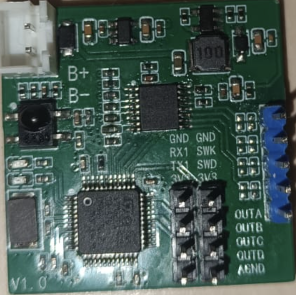
\includegraphics[width=\linewidth]{img/IR_receiver.png}
        \caption{Single IR receiver unit
        (\(2.5 \times 2.5\) cm)}
        \label{fig:single_receiver}
    \end{subfigure}
    \hfill
    \begin{subfigure}{0.48\textwidth}
        \centering
        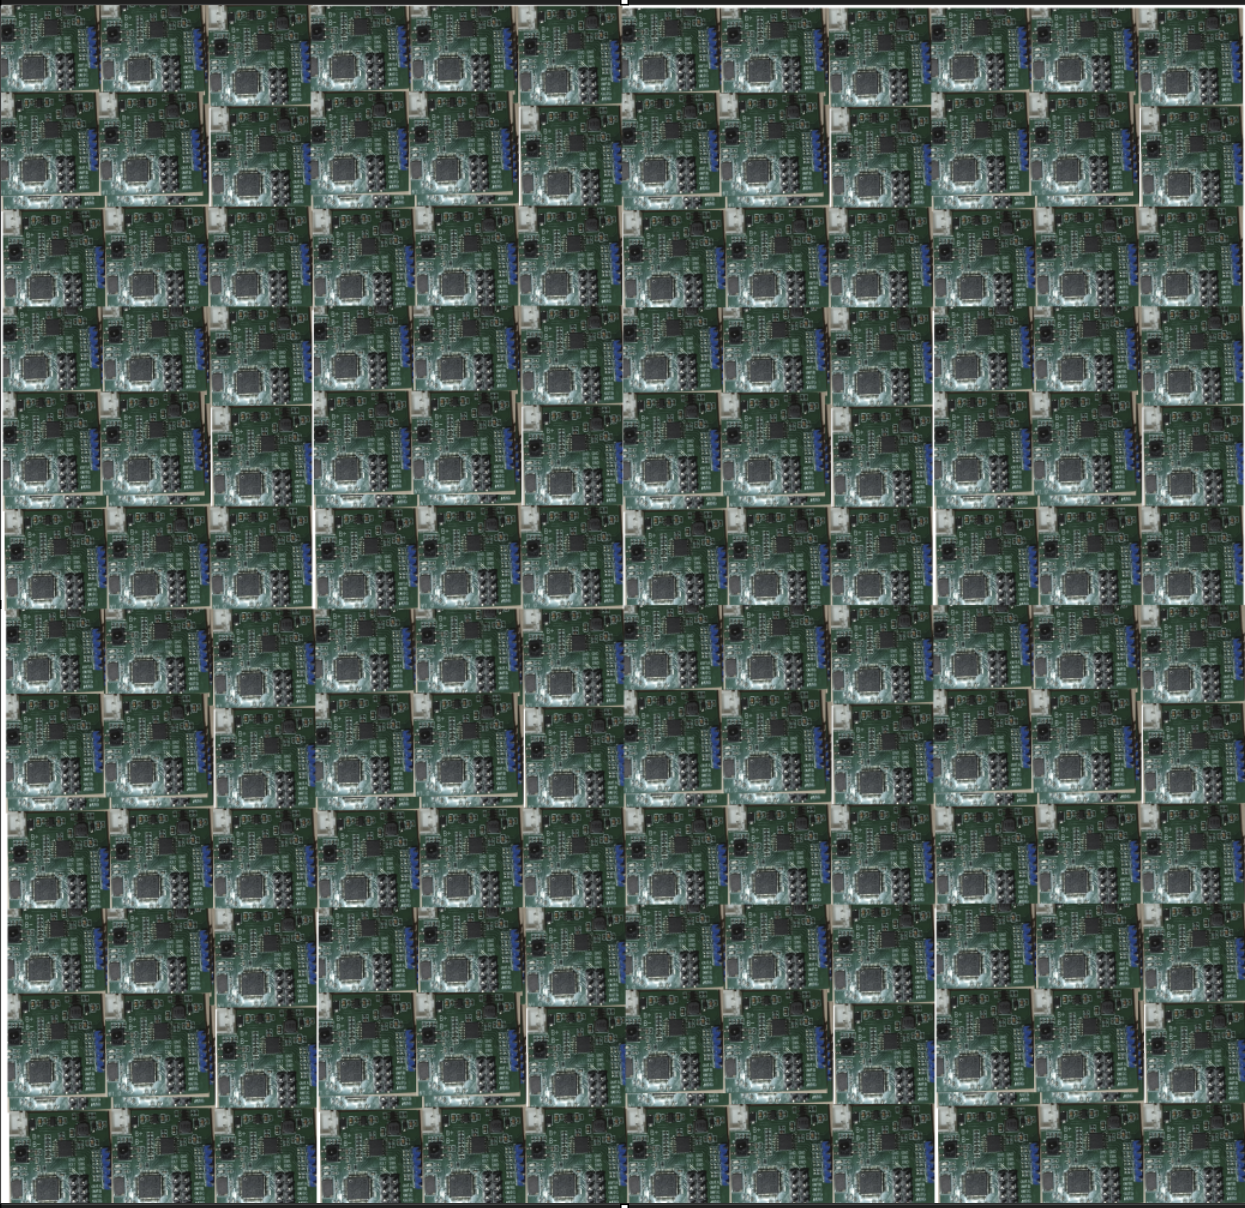
\includegraphics[width=\linewidth]{img/IR144.png}
        \caption{Complete \(12 \times 12\) receiver grid}
        \label{fig:receiver_grid}
    \end{subfigure}

    \caption{Infrared receiver configuration}
    \label{fig:ir_receiver_overview}

\end{figure}


% ============================================================
% 4.1 KY-005 LIMITATION
% ============================================================

\subsection{Limitations of the KY-005 Transmitter}

The initial experimental transmitter was the KY-005 infrared transmitter
module~\cite{arduino,sensorembedded}.

The module contains a conventional 5 mm infrared LED and is intended
primarily for short-range microcontroller applications.

Its approximate characteristics are summarized in
Table~\ref{tab:ky005}.

\begin{table}[H]
    \centering
    \caption{KY-005 Module Specifications}
    \label{tab:ky005}

    \begin{tabular}{@{}ll@{}}
        \toprule
        \textbf{Parameter} &
        \textbf{Value} \\
        \midrule

        Operating voltage &
        5 V \\

        Forward current &
        approximately 30--60 mA \\

        Power consumption &
        approximately 90 mW \\

        Operating temperature &
        \(-25^\circ\text{C}\) to \(80^\circ\text{C}\) \\

        Dimensions &
        \(18.5 \times 15\) mm \\

        \bottomrule
    \end{tabular}

\end{table}

Experimental testing showed that the KY-005 could not provide reliable
communication to all locations within the \(12 \times 12\) receiver
array at the intended operating distance.

The replacement transmitter must therefore provide greater useful
radiant intensity while maintaining an appropriate radiation pattern.


% ============================================================
% 5. OPTICAL GEOMETRY
% ============================================================

\section{Optical Geometry for 1--2 m Transmission}

The required beam angle can be estimated directly from the receiver
geometry.

The distance between the centre of the \(30 \times 30\) cm array and
one of its corners is

\[
r =
\sqrt{
(0.15)^2 + (0.15)^2
}
\]

which gives

\[
r \approx 0.212\,\text{m}.
\]

For a transmitter placed a perpendicular distance \(d\) from the
receiver plane, the angle between the optical axis and one corner is

\[
\alpha
=
\tan^{-1}
\left(
\frac{0.212}{d}
\right).
\]

Therefore, the required full angular coverage is approximately

\[
\theta_{\text{required}}
=
2\alpha
=
2\tan^{-1}
\left(
\frac{0.212}{d}
\right).
\]

The calculated values are shown in
Table~\ref{tab:beam_requirement}.

\begin{table}[H]
    \centering
    \caption{Required Beam Angle for the Receiver Array}
    \label{tab:beam_requirement}

    \begin{tabular}{@{}cc@{}}
        \toprule

        \textbf{Distance} &
        \textbf{Required Full Angle} \\

        \midrule

        1.0 m &
        \(24.0^\circ\) \\

        1.2 m &
        \(20.1^\circ\) \\

        1.5 m &
        \(16.1^\circ\) \\

        2.0 m &
        \(12.1^\circ\) \\

        \bottomrule
    \end{tabular}

\end{table}

These calculations show that the required beam is relatively narrow.
At a distance of 1 m, approximately \(24^\circ\) of full angular
coverage is sufficient to geometrically include the entire receiver
surface.

At 2 m, the required angle decreases to approximately \(12^\circ\).

The transmitter should therefore use a directional IR emitter rather
than a very wide radiation pattern. This concentrates a greater
fraction of the emitted infrared power toward the intended receiver
array and reduces unnecessary optical spill.


% ============================================================
% 6. LED SELECTION
% ============================================================

\section{Infrared Emitter Selection}

Two Vishay 940 nm infrared emitters were considered:

\begin{itemize}
    \item TSAL6200;
    \item TSAL6100.
\end{itemize}

Both devices are designed for infrared free-air transmission and have
fast optical switching characteristics suitable for a 38 kHz carrier
\cite{tsal6200,tsal6100}.

Their main characteristics are compared in
Table~\ref{tab:led_comparison}.

\begin{table}[H]
    \centering
    \caption{Comparison of Candidate 940 nm Infrared Emitters}
    \label{tab:led_comparison}

    \begin{tabular}{@{}lcc@{}}
        \toprule

        \textbf{Parameter} &
        \textbf{TSAL6200} &
        \textbf{TSAL6100} \\

        \midrule

        Peak wavelength &
        940 nm &
        940 nm \\

        Angle of half intensity &
        \(\pm17^\circ\) &
        \(\pm10^\circ\) \\

        Approx. full half-intensity angle &
        \(34^\circ\) &
        \(20^\circ\) \\

        Typical radiant intensity at 100 mA &
        72 mW/sr &
        170 mW/sr \\

        Typical forward voltage at 100 mA &
        1.35 V &
        1.35 V \\

        Maximum forward current &
        100 mA &
        100 mA \\

        Typical rise time &
        15 ns &
        15 ns \\

        Typical fall time &
        15 ns &
        15 ns \\

        \bottomrule
    \end{tabular}

\end{table}


% ============================================================
% 6.1 PRIMARY EMITTER
% ============================================================

\subsection{TSAL6200 as the Primary Emitter}

The TSAL6200 is selected as the primary emitter.

Its nominal angle of half intensity is

\[
\phi = \pm17^\circ.
\]

The diameter corresponding to this half-intensity cone at distance
\(d\) is approximately

\[
D =
2d\tan(17^\circ).
\]

At 1 m,

\[
D_{1\,\text{m}}
=
2(1)\tan(17^\circ)
\approx
0.61\,\text{m}.
\]

At 2 m,

\[
D_{2\,\text{m}}
=
2(2)\tan(17^\circ)
\approx
1.22\,\text{m}.
\]

The receiver array has a width of only 0.30 m.
Consequently, all four corners of the receiver array lie inside the
nominal half-intensity cone at the minimum expected operating distance
of approximately 1 m.

This provides useful alignment margin while remaining considerably
more directional than a wide-angle infrared emitter.


% ============================================================
% 6.2 ALTERNATIVE EMITTER
% ============================================================

\subsection{TSAL6100 as a Narrow-Beam Alternative}

The TSAL6100 has an angle of half intensity of approximately

\[
\pm10^\circ
\]

and a typical radiant intensity of approximately

\[
170\,\text{mW/sr}
\]

at 100 mA.

Its narrower radiation pattern produces greater axial radiant intensity
and may therefore be advantageous when longer transmission range or
lower optical spill is required.

At a distance of 1 m, the corners of the receiver array are located at
approximately

\[
\tan^{-1}
\left(
\frac{0.212}{1}
\right)
\approx
12^\circ
\]

from the optical axis.

The receiver corners therefore lie slightly outside the TSAL6100
nominal \(\pm10^\circ\) half-intensity cone at 1 m.

At approximately 1.2 m and greater distances, the required corner angle
becomes close to or smaller than \(10^\circ\).

For this reason, the TSAL6100 will be treated as an experimental
alternative, particularly for longer-distance and low-interference
tests.


% ============================================================
% 7. MULTI-LED TRANSMITTER
% ============================================================

\section{Multi-LED Transmitter Architecture}

The transmitter is designed around series-connected pairs of IR LEDs.

The basic configuration contains:

\[
2 \times \text{TSAL6200}.
\]

The two LEDs are connected in series and therefore carry the same
current.

A second identical branch may be populated if additional optical
output is required.

The fully populated configuration therefore consists of

\[
4 \times \text{TSAL6200}
\]

arranged as two parallel branches, with two LEDs in series in each
branch.

Each parallel branch has its own current-limiting resistor.

This is necessary because small differences in LED forward voltage
can otherwise produce unequal current distribution between parallel
LED paths.


% ============================================================
% 8. DRIVER CIRCUIT
% ============================================================

\section{MOSFET Driver Circuit}

The 3.3 V FPGA output is used only as a control signal.
The LED current is supplied from an external regulated 5 V supply.

An AO3400A logic-level N-channel MOSFET is used as the low-side switch
\cite{ao3400a}.

The AO3400A is suitable for direct control from low-voltage digital
logic because its drain-source on-resistance is specified at gate
voltages as low as 2.5 V.

The proposed circuit is shown in
\begin{figure}[H]
    \centering
    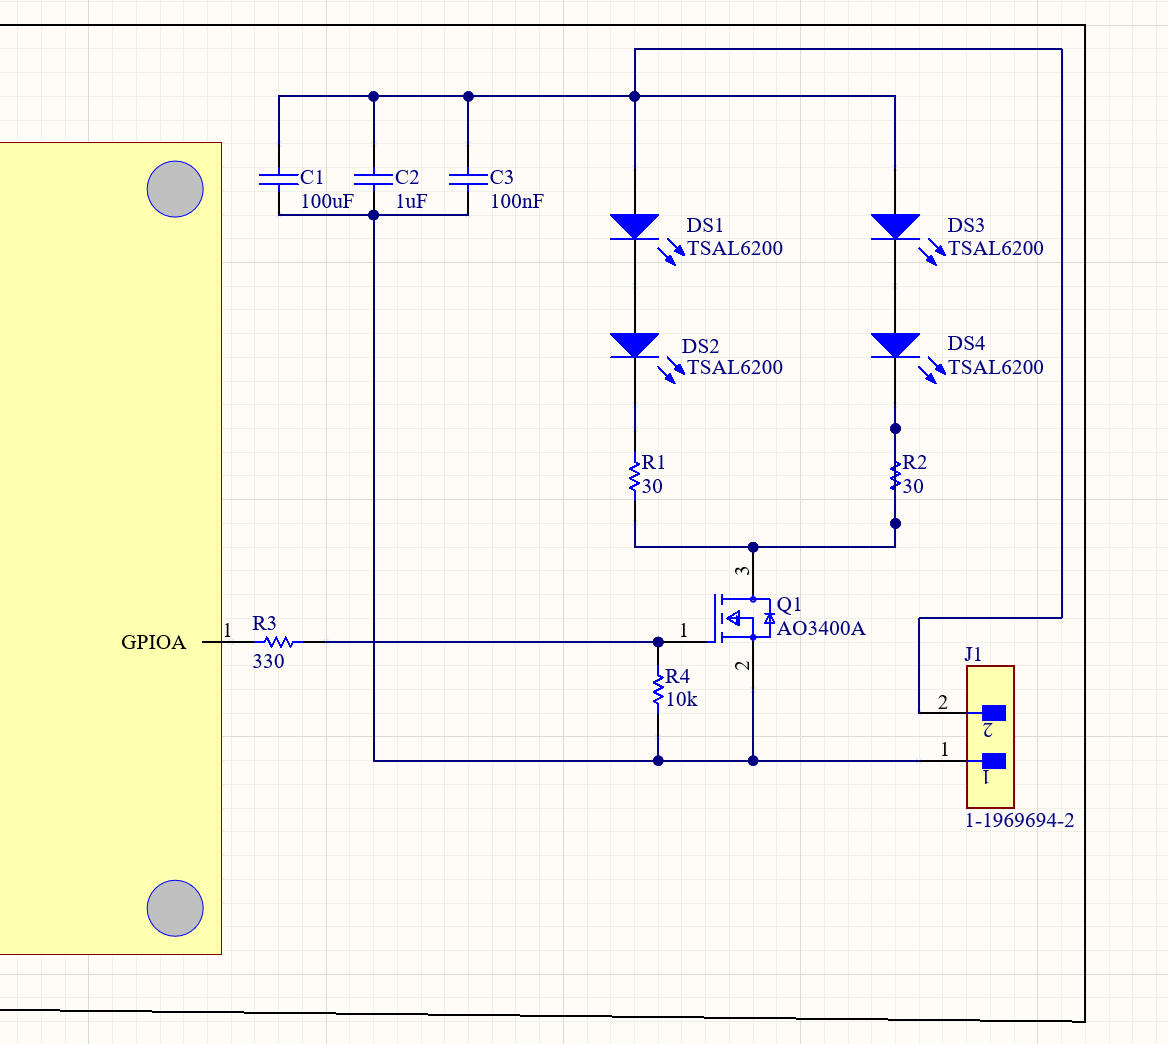
\includegraphics[width=1\linewidth]{img/New_Driving_Circuit.png}
\end{figure}
\subsection{Single-Emitter Transmitter Circuit}

As an additional experimental configuration, a transmitter channel can use
only one TSAL6200 emitter instead of the two-LED series branch. The rest of
the driver remains unchanged: the AO3400A is used as the low-side switch,
the FPGA drives the gate through a \(330\,\Omega\) resistor, and a
\(10\,\text{k}\Omega\) pull-down resistor keeps the MOSFET OFF during
startup.

For a single TSAL6200 on a regulated 5 V supply, the LED current-limiting
resistor is increased from \(30\,\Omega\) to \(47\,\Omega\). Using
\(V_F \approx 1.35\,\text{V}\),

\[
I_F \approx
\frac{5-1.35}{47}
\approx
77.7\,\text{mA}.
\]

The corresponding instantaneous resistor dissipation is

\[
P_R = I_F^2R
\approx
(0.0777)^2(47)
\approx
0.28\,\text{W},
\]

therefore a \(47\,\Omega,\ 0.5\,\text{W}\) resistor is suitable for the
prototype.

This single-emitter version is useful as a minimum-power test configuration.
If one LED already provides reliable decoding at the required receiver
positions, there is no reason to add unnecessary optical power. A single
emitter does not eliminate interference from other independent
transmitters, but the lower optical output can reduce unwanted illumination
of neighboring receiver regions.

\begin{figure}[H]
    \centering
    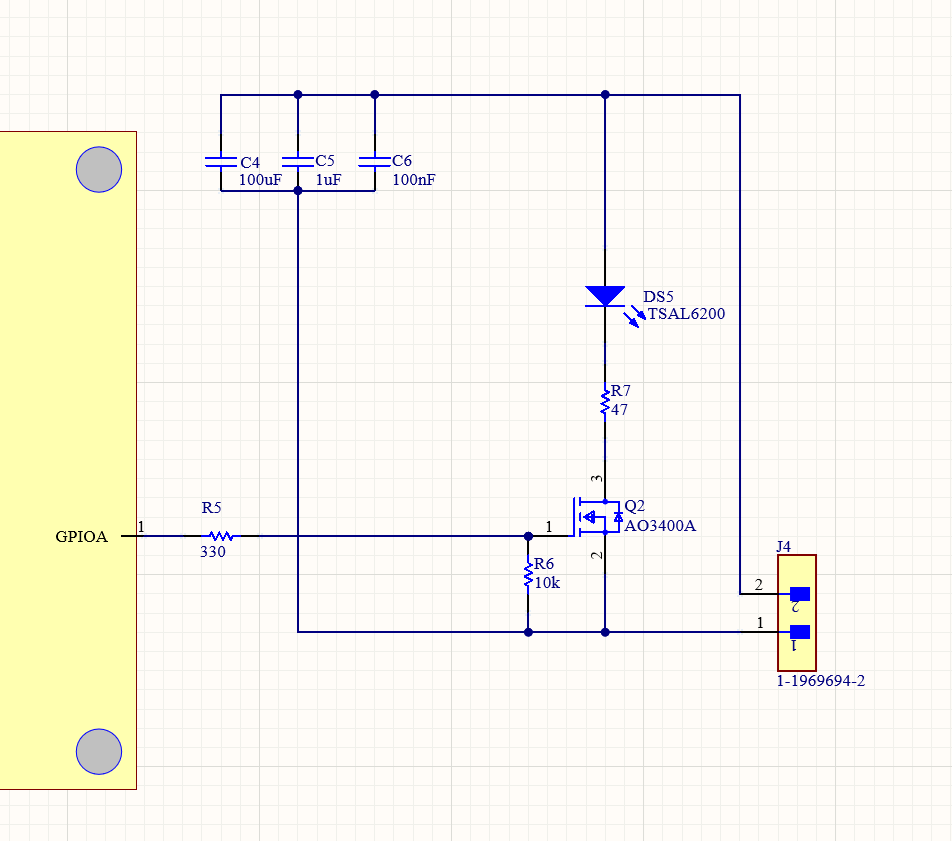
\includegraphics[width=1\linewidth]{img/Driving circuit one.png}
    \caption{Single-emitter transmitter circuit using one TSAL6200 and a
    \(47\,\Omega\) current-limiting resistor.}
    \label{fig:single_emitter_circuit}
\end{figure}
% ============================================================
% 9. COMPONENTS
% ============================================================

\subsection{Circuit Component Specifications}

The proposed component values are summarized in
Table~\ref{tab:circuit_components}.

\begin{table}[H]
    \centering
    \caption{Transmitter Circuit Components}
    \label{tab:circuit_components}

    \begin{tabular}{@{}p{3.1cm}p{4.1cm}p{5.7cm}@{}}
        \toprule

        \textbf{Component} &
        \textbf{Value / Part} &
        \textbf{Purpose} \\

        \midrule

        IR emitters &
        TSAL6200 \cite{tsal6200} &
        940 nm directional optical transmission  \\

        Alternative emitter &
        TSAL6100 \cite{tsal6100}  &
        Narrower beam for comparison testing \\

        MOSFET \(Q_1\) &
        AO3400A \cite{ao3400a} &
        Logic-level low-side switch \\

        \(R_G\) &
        \(330\,\Omega\), 1/4 W \cite{Rg}&
        Limits transient FPGA gate charging current \\

        \(R_{PD}\) &
        \(10\,\text{k}\Omega\), 1/4 W \cite{Rpd} &
        Holds MOSFET OFF during FPGA startup \\

        \(R_{S1}\), \(R_{S2}\) &
        \(30\,\Omega\), 0.5 W \cite{RS} &
        Sets current independently in each LED branch \\

        Single-emitter test resistor &
        \(47\,\Omega\), 0.5 W &
        Sets approximately \(78\,\text{mA}\) with one TSAL6200 on 5 V \\

        \(C_1\) &
        \(100\,\mu\text{F}\), 10 V or greater &
        Local energy storage \\

        \(C_2\) &
        \(1\,\mu\text{F}\) ceramic &
        Local supply decoupling \\

        \(C_3\) &
        \(100\,\text{nF}\) ceramic &
        High-frequency supply decoupling \\

        Power supply &
        Regulated 5 V DC &
        Powers LED branches \\

        Control input &
        3.3 V FPGA logic &
        NEC-modulated 38 kHz switching signal \\

        \bottomrule
    \end{tabular}

\end{table}


% ============================================================
% 10. CURRENT CALCULATIONS
% ============================================================

\subsection{LED Branch Current Calculation}

The typical forward voltage of the TSAL6200 at approximately 100 mA is

\[
V_F \approx 1.35\,\text{V}.
\]

Because two emitters are connected in series,

\[
V_{\text{LED,string}}
=
2V_F
\]

and therefore

\[
V_{\text{LED,string}}
=
2(1.35)
=
2.70\,\text{V}.
\]

The AO3400A voltage drop at the expected current is small compared with
the supply voltage, so the nominal branch current can initially be
estimated as

\[
I_F
\approx
\frac{
V_{\text{supply}} - 2V_F
}{
R_S
}.
\]

Using

\[
V_{\text{supply}}=5\,\text{V}
\]

and

\[
R_S=30\,\Omega,
\]

the nominal current becomes

\[
I_F
\approx
\frac{
5 - 2(1.35)
}{
30
}
\]

which gives

\[
I_F
\approx
76.7\,\text{mA}.
\]

Therefore, the nominal branch current is approximately

\[
\boxed{
I_F \approx 77\,\text{mA}
}.
\]

The two LEDs in one series branch both carry this same current.


\subsection{Single-Emitter Current Calculation}

For the single-emitter configuration shown in
Figure~\ref{fig:single_emitter_circuit}, only one TSAL6200 is present in the
LED current path. To keep approximately the same LED current, the resistor
must therefore be changed to \(47\,\Omega\):

\[
I_{F,\text{single}}
\approx
\frac{5-1.35}{47}
\approx
77.7\,\text{mA}.
\]

Using the original \(30\,\Omega\) resistor with only one LED would instead
give approximately

\[
\frac{5-1.35}{30}
\approx
122\,\text{mA},
\]

which is above the intended continuous-current operating point used in this
design. The single-emitter prototype therefore uses
\(47\,\Omega,\ 0.5\,\text{W}\).


% ============================================================
% 11. FULLY POPULATED CURRENT
% ============================================================

\subsection{Current with Two LED Branches}

When both LED branches are populated, each branch carries approximately

\[
77\,\text{mA}.
\]

Therefore, when the MOSFET is ON,

\[
I_{\text{total}}
\approx
2(77\,\text{mA})
\]

or

\[
\boxed{
I_{\text{total}}
\approx
154\,\text{mA}
}.
\]

The actual current should be measured during prototype testing because
LED forward voltage varies between devices and with temperature.


% ============================================================
% 12. RESISTOR DISSIPATION
% ============================================================

\subsection{Current-Limiting Resistor Dissipation}

The instantaneous power dissipated by each current-limiting resistor is

\[
P_R =
I^2R.
\]

Using

\[
I = 0.077\,\text{A}
\]

and

\[
R = 30\,\Omega,
\]

gives

\[
P_R
=
(0.077)^2(30)
\]

and therefore

\[
P_R
\approx
0.178\,\text{W}.
\]

A \(0.5\,\text{W}\) resistor provides sufficient nominal power margin.

Because the LEDs are modulated according to NEC carrier bursts, the
long-term average dissipation is lower than the instantaneous value.


% ============================================================
% 13. MOSFET LOSS
% ============================================================

\subsection{MOSFET Conduction Loss}

The AO3400A has a specified maximum

\[
R_{\text{DS(on)}}
\approx
48\,\text{m}\Omega
\]

at

\[
V_{\text{GS}} = 2.5\,\text{V}.
\]

For the fully populated transmitter,

\[
I_D \approx 0.154\,\text{A}.
\]

The approximate MOSFET conduction loss is

\[
P_Q =
I_D^2 R_{\text{DS(on)}}.
\]

Therefore,

\[
P_Q
=
(0.154)^2(0.048)
\]

which gives approximately

\[
P_Q
\approx
1.1\,\text{mW}.
\]

The MOSFET conduction loss is therefore very small for the expected
operating current.


% ============================================================
% 14. SWITCHING SPEED
% ============================================================

\subsection{Switching-Speed Requirement}

The NEC carrier period is approximately

\[
T_c = 26.3\,\mu\text{s}.
\]

The TSAL6200 has typical optical rise and fall times of approximately

\[
t_r \approx 15\,\text{ns}
\]

and

\[
t_f \approx 15\,\text{ns}.
\]

The ratio between the optical rise time and carrier period is

\[
\frac{
15\,\text{ns}
}{
26.3\,\mu\text{s}
}
\approx
5.7\times10^{-4}.
\]

The emitter switching time is therefore negligible compared with the
38 kHz carrier period.

For this application, optical coverage and radiant intensity are more
significant design parameters than LED switching speed.


% ============================================================
% 15. CONNECTIONS
% ============================================================

\subsection{Connection Instructions}

The transmitter should be connected as follows:

\begin{enumerate}

    \item Connect the external regulated +5 V supply to the first IR
    LED in each populated branch.

    \item Connect two TSAL6200 emitters in series in each branch.

    \item Install a separate \(30\,\Omega\), 0.5 W resistor in each
    branch.

    \item Connect the lower ends of the two branches to the drain of
    the AO3400A.

    \item Connect the AO3400A source directly to ground.

    \item Connect the FPGA output to the MOSFET gate through a
    \(330\,\Omega\) resistor.

    \item Connect a \(10\,\text{k}\Omega\) pull-down resistor between
    the MOSFET gate and ground.

    \item Connect the FPGA ground and the external 5 V power-supply
    ground together.

    \item Place the \(100\,\mu\text{F}\), \(1\,\mu\text{F}\), and
    \(100\,\text{nF}\) bypass capacitors between +5 V and ground close
    to the LED branches and MOSFET.

\end{enumerate}


% ============================================================
% 16. OPERATION
% ============================================================

\subsection{Operating Principle}

The FPGA generates the NEC waveform containing the 38 kHz carrier.

When the FPGA output is HIGH, the AO3400A gate is driven to approximately
3.3 V relative to its grounded source.

The MOSFET turns ON, allowing current to flow through each populated
LED branch:

\[
+5\,\text{V}
\rightarrow
LED
\rightarrow
LED
\rightarrow
R_S
\rightarrow
Q_1
\rightarrow
\text{GND}.
\]

The infrared emitters therefore generate the optical carrier.

When the FPGA output becomes LOW, the MOSFET turns OFF and current
through the LED branches stops.

The \(10\,\text{k}\Omega\) gate pull-down resistor ensures that the
MOSFET remains OFF when the FPGA output is unconfigured, such as during
startup or reset.

The gate resistor reduces the short transient current required to
charge and discharge the MOSFET gate capacitance.


% ============================================================
% 17. DECOUPLING
% ============================================================

\subsection{Power-Supply Decoupling}

Fast switching of the IR LED current produces transient changes in
supply current.

Local bypass capacitors are therefore placed near the transmitter
circuit.

The proposed capacitor network contains:

\[
C_1 = 100\,\mu\text{F},
\]

\[
C_2 = 1\,\mu\text{F},
\]

and

\[
C_3 = 100\,\text{nF}.
\]

The larger capacitor provides local energy storage while the smaller
ceramic capacitors suppress higher-frequency supply disturbances.

PCB traces between these capacitors, the LED branches, and the MOSFET
should be kept short.


% ============================================================
% 18. POWER SUPPLY
% ============================================================

\subsection{Power-Supply Requirement}

A single fully populated transmitter is expected to draw approximately

\[
154\,\text{mA}
\]

during the ON portion of the carrier waveform.

A regulated 5 V, 1 A supply therefore provides substantial current
margin for a single experimental transmitter.

When multiple transmitters share a common supply, the required supply
current depends on the maximum number of simultaneously active
transmitters.

For example, if all 24 transmitters were fully populated and switched
ON simultaneously, the instantaneous LED current would be approximately

\[
I_{\text{system}}
=
24(0.154)
\]

which gives

\[
I_{\text{system}}
\approx
3.7\,\text{A}.
\]

This value represents an instantaneous upper-bound estimate for the
LED transmitter circuits only.

A shared supply should therefore include additional margin for the
control electronics, wiring losses, transient current, and other system
loads.


% ============================================================
% 19. THERMAL CHECK
% ============================================================

\subsection{Thermal Considerations}

The emitter branches operate below the 100 mA forward-current rating of
the selected IR LEDs.

The current-limiting resistors dissipate approximately 0.18 W during
the ON state, while the calculated AO3400A conduction loss is only on
the order of 1 mW.

The NEC waveform additionally reduces average dissipation because the
LEDs are not continuously energized.

Normal PCB spacing and ventilation are therefore expected to be
adequate for the prototype.

Component temperature should nevertheless be checked during initial
continuous testing.


% ============================================================
% 20. INTERFERENCE
% ============================================================

\section{Multi-Transmitter Interference}

Multiple LEDs connected to the same switching circuit and carrying the
same NEC signal behave as one optical transmitter. Adding LEDs in this
case increases the available optical output without introducing a new
data signal.

A different situation occurs when independent transmitters send
different NEC messages simultaneously.

Because the transmitters use the same 940 nm optical region and the
same 38 kHz carrier, radiation from more than one transmitter may reach
the same receiver.

The receiver cannot identify the physical origin of overlapping
38 kHz optical signals solely from their carrier frequency.
Simultaneous signals may therefore corrupt the received NEC waveform.

For this reason, transmitter directivity is an important part of the
system design.

The proposed directional emitters reduce interference by concentrating
the radiation toward the intended receiver area.


% ============================================================
% 20.1 SPATIAL ISOLATION
% ============================================================

\subsection{Spatial Isolation}

Spatial isolation can be improved through several methods:

\begin{itemize}

    \item selecting an appropriate emitter beam angle;

    \item physically separating adjacent transmitters;

    \item carefully orienting each transmitter toward its intended
    receiver region;

    \item using opaque tubes or barriers around the emitters;

    \item reducing optical output to the minimum level required for
    reliable communication.

\end{itemize}

Using the minimum necessary optical output is particularly important.
Once reliable decoding is achieved at the worst-position receiver,
additional optical power may increase interference without improving
the useful communication link.


% ============================================================
% 21. PROTOTYPE PROCEDURE
% ============================================================

\section{Prototype and Experimental Procedure}

The transmitter PCB should support four IR LED positions arranged as
two independently current-limited series branches.

The initial prototype should populate only one branch containing two
TSAL6200 emitters.

The following measurements should then be performed:

\begin{enumerate}

    \item First test the single-emitter configuration using one TSAL6200,
    a \(47\,\Omega,\ 0.5\,\text{W}\) resistor, and approximately
    \(78\,\text{mA}\) LED current. If this configuration already gives
    reliable reception at the required receiver positions, record it as the
    minimum-power operating point.

    \item Operate two TSAL6200 emitters at approximately
    \(77\,\text{mA}\).

    \item Position the transmitter approximately 1.0 m from the receiver
    array.

    \item Verify NEC reception at the centre of the array.

    \item Verify reception at the four edge-centre positions.

    \item Verify reception at the four corners of the array.

    \item Repeat the measurements at approximately 1.5 m.

    \item Repeat the measurements at approximately 2.0 m.

    \item If reception margin is insufficient, populate the second
    two-LED branch.

    \item Repeat the complete distance and position measurements using
    four emitters.

    \item Compare the TSAL6200 configuration with the narrower-beam
    TSAL6100 configuration.

\end{enumerate}


% ============================================================
% 21.1 SUCCESS CRITERION
% ============================================================

\subsection{Receiver Coverage Criterion}

The transmitter should not be evaluated only at the centre of the
receiver grid.

Reliable operation should be verified at the positions where optical
intensity is expected to be lowest, particularly the four corners.

The transmitter will be considered to provide sufficient optical
coverage if all tested receiver positions can decode the NEC signal
reliably at the required operating distance.

The desired operating point is therefore the lowest optical output
that provides adequate decoding margin at the worst-case receiver
location.


% ============================================================
% 21.2 INTERFERENCE TEST
% ============================================================

\subsection{Interference Test}

After single-transmitter operation has been validated, two adjacent
transmitters should be tested together.

Testing should include:

\begin{enumerate}

    \item only transmitter A active;

    \item only transmitter B active;

    \item A and B transmitting at different times;

    \item A and B transmitting simultaneously;

    \item different physical separation between the transmitters;

    \item different transmitter orientations;

    \item optional optical barriers or guiding tubes.

\end{enumerate}

The experiment should determine whether narrower radiation patterns
or physical isolation significantly reduce cross-channel interference.


% ============================================================
% 22. TSAL6100 COMPARISON TEST
% ============================================================

\subsection{Beam-Angle Comparison Experiment}

The TSAL6200 and TSAL6100 provide an opportunity to experimentally
study the trade-off between beam width and radiant intensity.

The TSAL6200 provides a wider

\[
\pm17^\circ
\]

half-intensity angle, whereas the TSAL6100 provides a narrower

\[
\pm10^\circ
\]

half-intensity angle.

The narrower emitter produces greater axial radiant intensity but is
more sensitive to alignment.

For each emitter type, the following should be measured:

\begin{itemize}

    \item maximum reliable communication distance;

    \item reliability at receiver-array corners;

    \item tolerance to lateral transmitter misalignment;

    \item interference observed at neighboring receivers.

\end{itemize}

These measurements will determine which radiation pattern provides the
best compromise between receiver coverage and transmitter isolation.


% ============================================================
% 23. PCB CONSIDERATIONS
% ============================================================

\section{PCB Design Considerations}

The transmitter PCB should provide four emitter footprints.

The emitters should be positioned symmetrically around the optical
centre of the transmitter so that multiple LEDs illuminate
approximately the same receiver region.

The two LED branches should have identical trace geometry where
practical.

The AO3400A and bypass capacitors should be positioned close to the LED
branches to minimize switching-loop area.

The ground path between the MOSFET and power supply should have low
impedance.

The FPGA control trace does not carry the LED current and may therefore
be routed separately from the power path.

Where transmitter interference is significant, mechanical mounting
should permit adjustment of the emitter orientation.


% ============================================================
% 24. DESIGN SUMMARY
% ============================================================

\section{Proposed Transmitter Configuration}

The baseline transmitter configuration is summarized in
Table~\ref{tab:design_summary}.

\begin{table}[H]
    \centering
    \caption{Proposed IR Transmitter Configuration}
    \label{tab:design_summary}

    \begin{tabular}{@{}ll@{}}
        \toprule

        \textbf{Parameter} &
        \textbf{Design Value} \\

        \midrule

        IR wavelength &
        940 nm \\

        Protocol &
        NEC \\

        Carrier frequency &
        38 kHz \\

        Operating distance &
        approximately 1--2 m \\

        Receiver area &
        \(30 \times 30\) cm \\

        Primary emitter &
        Vishay TSAL6200 \\

        Emitter angle of half intensity &
        \(\pm17^\circ\) \\

        Initial emitter count &
        2 \\

        Maximum prototype emitter count &
        4 \\

        LED arrangement &
        2 LEDs per series branch \\

        Number of branches &
        1 initially, 2 optional \\

        Nominal branch current &
        approximately 77 mA \\

        MOSFET &
        AO3400A \\

        Supply voltage &
        5 V \\

        FPGA control voltage &
        3.3 V \\

        Branch resistor &
        \(30\,\Omega,\ 0.5\,\text{W}\) \\

        Single-emitter test configuration &
        1 TSAL6200 with \(47\,\Omega,\ 0.5\,\text{W}\) \\

        Gate resistor &
        \(330\,\Omega\) \\

        Gate pull-down &
        \(10\,\text{k}\Omega\) \\

        \bottomrule
    \end{tabular}

\end{table}


% ============================================================
% 25. CONCLUSION
% ============================================================

\section{Conclusion}

A directional 940 nm infrared transmitter has been proposed for
communication with a \(12 \times 12\) receiver array located
approximately 1--2 m from the transmitter.

Geometrical analysis shows that the complete \(30 \times 30\) cm
receiver array requires approximately \(24^\circ\) of full angular
coverage at 1 m and only approximately \(12^\circ\) at 2 m.

The Vishay TSAL6200, with an angle of half intensity of approximately
\(\pm17^\circ\), provides suitable coverage margin for this distance
range while maintaining substantially greater directionality than a
very wide-beam emitter.

Two TSAL6200 emitters connected in series form the baseline
configuration. A second identical branch allows the transmitter to be
expanded to four emitters if experimental measurements show that
additional optical output is required.

The emitters are controlled using an AO3400A N-channel MOSFET driven by
the FPGA's 3.3 V NEC signal. Each LED branch includes its own
current-limiting resistor and operates at a nominal current of
approximately 77 mA.

The final number of emitters should be determined experimentally by
testing the centre, edges, and corners of the receiver array at
1.0 m, 1.5 m, and 2.0 m.

A single-emitter TSAL6200 configuration with a
\(47\,\Omega,\ 0.5\,\text{W}\) resistor is also included as a minimum-power
test case. If it provides reliable decoding at the required distance, it can
reduce unnecessary optical spill compared with the higher-output
configurations.

The same test platform can also compare the wider TSAL6200 with the
narrower TSAL6100 and quantify the trade-off between receiver coverage,
radiant intensity, alignment tolerance, and interference between
neighboring transmitters.


% ============================================================
% BIBLIOGRAPHY
% ============================================================

\begin{thebibliography}{9}

\bibitem{medium}
BlueEast.
\emph{NEC Transmission Protocol for Air Conditioners}.
\\
\url{https://medium.com/blueeast/nec-transmission-protocol-for-air-conditioners-67c8a698e633}

\bibitem{edmund}
Edmund Optics.
\emph{The Correct Material for Infrared Applications}.
\\
\url{https://www.edmundoptics.com/knowledge-center/application-notes/optics/the-correct-material-for-infrared-applications/}

\bibitem{arduino}
ArduinoModules.info.
\emph{KY-005 Infrared Transmitter Sensor Module}.
\\
\url{https://arduinomodules.info/ky-005-infrared-transmitter-sensor-module/}

\bibitem{sensorembedded}
Sensor Embedded.
\emph{KY-005 38 kHz Infrared Transmit Sensor Module}.
\\
\url{https://www.mouser.hk/en/ProductDetail/Vishay-Semiconductors/TSAL6200?qs=GAjK1cmKyrlKVEUhArzG2A%3D%3D}

\bibitem{tsal6200}
Vishay Semiconductors.
\emph{TSAL6200 Datasheet: 940 nm Infrared Emitting Diode}.
\\
\url{https://www.vishay.com/docs/81010/tsal6200.pdf}

\bibitem{tsal6100}
Vishay Semiconductors.
\emph{TSAL6100 Datasheet: 940 nm Infrared Emitting Diode}.
\\
\url{http://mouser.hk/en/ProductDetail/Vishay-Semiconductors/TSAL6100?qs=hQ8xas2ojoxzFnfG3K8LcA%3D%3D}

\bibitem{ao3400a}
Alpha \& Omega Semiconductor.
\emph{AO3400A 30 V N-Channel MOSFET}.
\\
\url{https://www.digikey.hk/en/products/detail/alpha-omega-semiconductor-inc/AO3400A/1855772?srsltid=AfmBOopS0N42zk652V4eP_M87ckK7aip--HF6o5p8eZQwwIq4RlECrnc}
\bibitem{RS}
\(30\,\Omega\) 0.5W Resistor
\emph{352130RFT 0.5W \(30\,\Omega\) }.
\\
\url{https://www.digikey.hk/en/products/detail/te-connectivity-passive-product/352130RFT/4279927?utm_source=chatgpt.com}
\bibitem{Rpd}
\(330\,\Omega\) Resistor 
\emph{CF14JT330R \(330\,\Omega\)}.
\\
\url{https://www.digikey.hk/en/products/detail/stackpole-electronics-inc/CF14JT330R/1830338?utm_source=chatgpt.com}
\bibitem{Rg}
\(10k\,\Omega\) Resistor 
\emph{CF14JT10K0 \(10k\,\Omega\)}.
\\
\url{https://www.digikey.hk/en/products/detail/stackpole-electronics-inc/CF14JT10K0/CF14JT10K0CT-ND/1830374?utm_source=chatgpt.com}
\end{thebibliography}

\end{document}